\begin{figure*}[!t]
	\begin{center}
		\subfigure[No Failure]
		{
			\label{fig:sc_no_fail}
			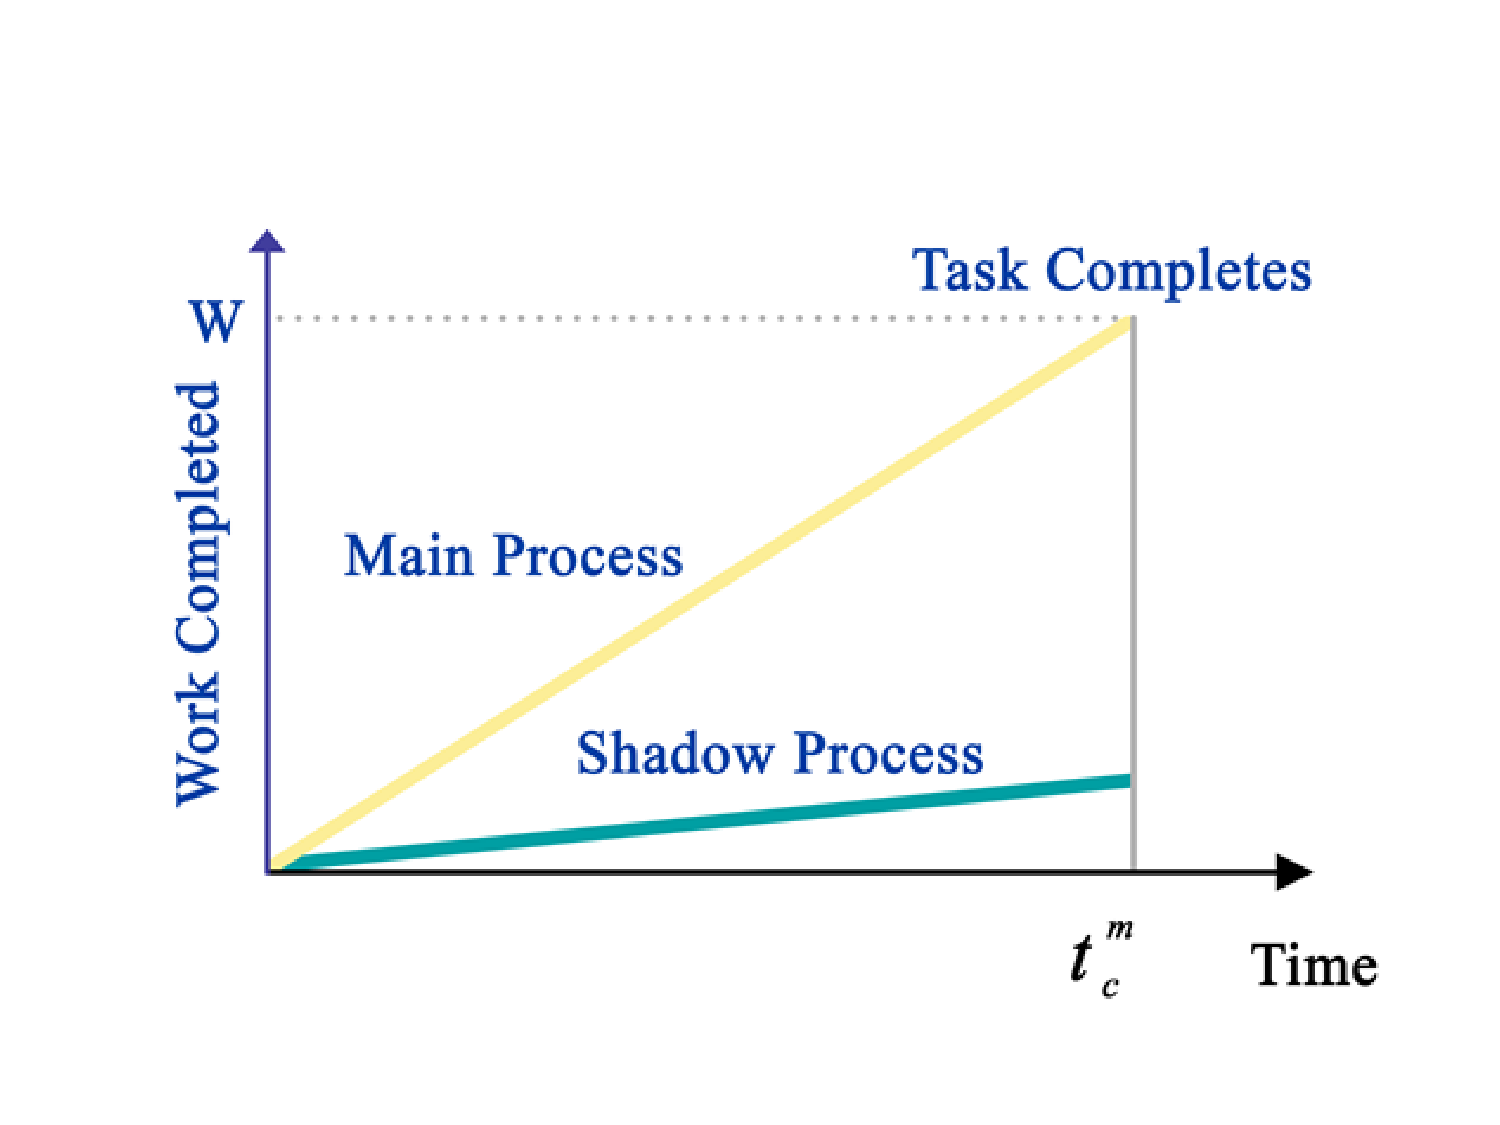
\includegraphics[width=0.32\textwidth]{diagrams/example1.pdf}
		}
		\subfigure[Shadow Process Failure]
		{
			\label{fig:sc_shadow_fail}
			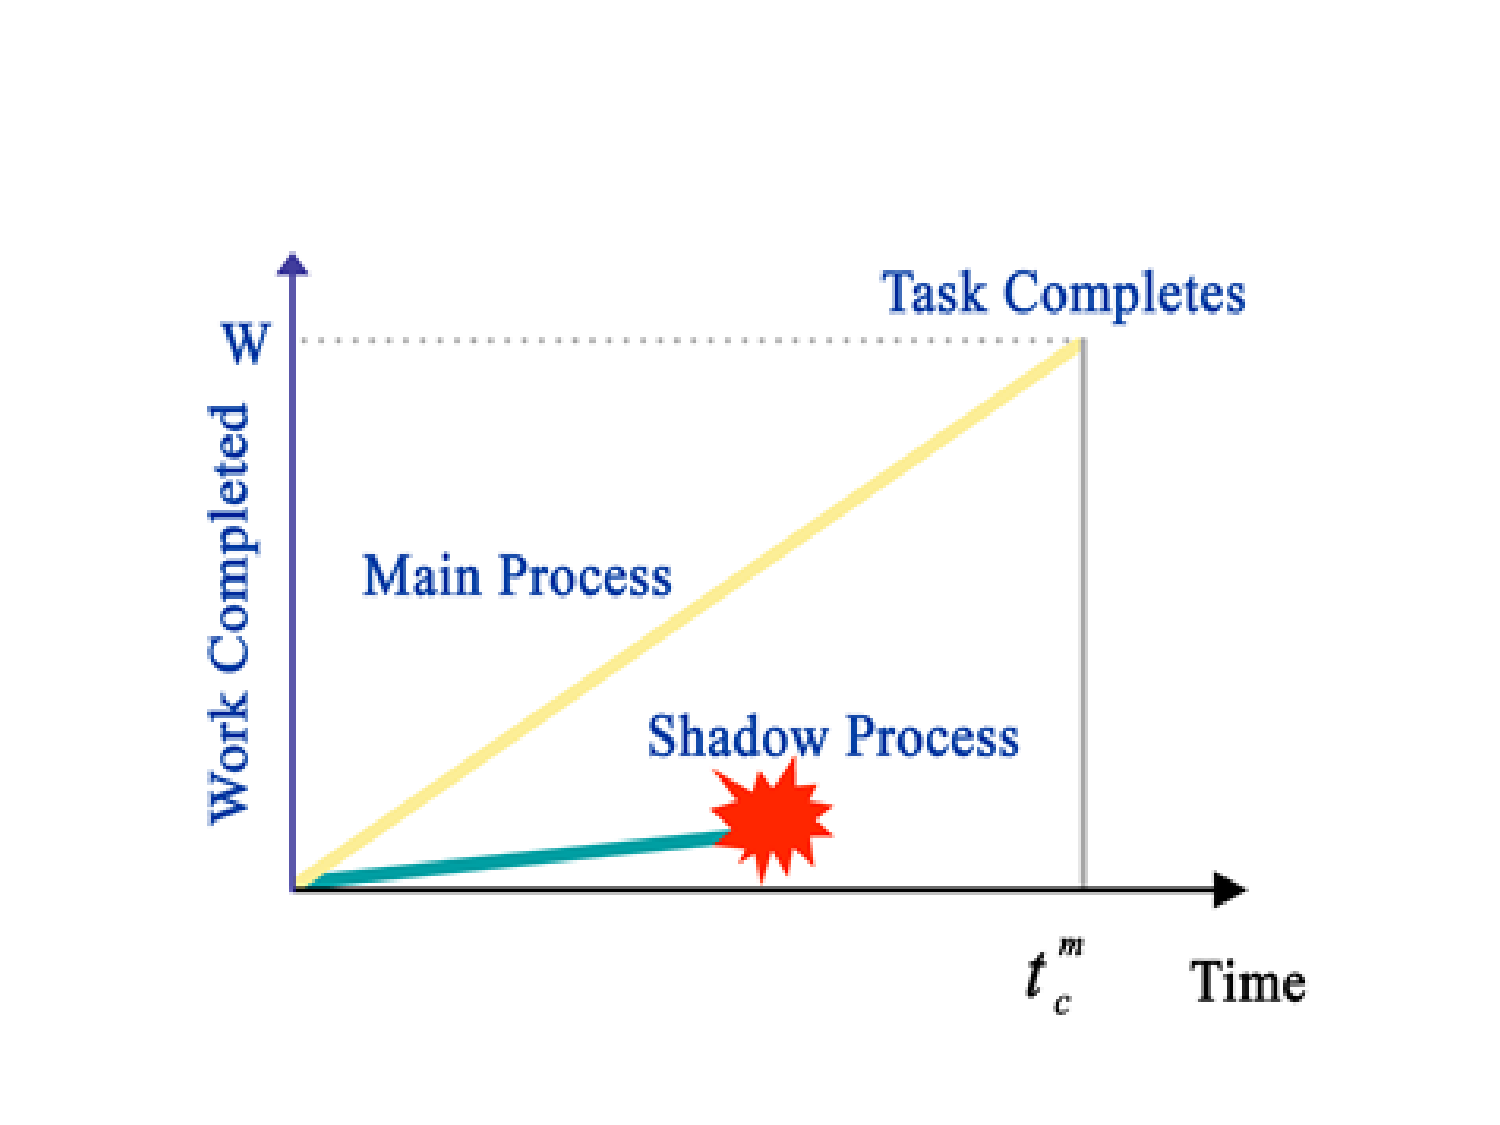
\includegraphics[width=0.29\textwidth]{diagrams/example3.pdf}
		}
		\subfigure[Main Process Failure]
		{
			\label{fig:sc_main_fail}
			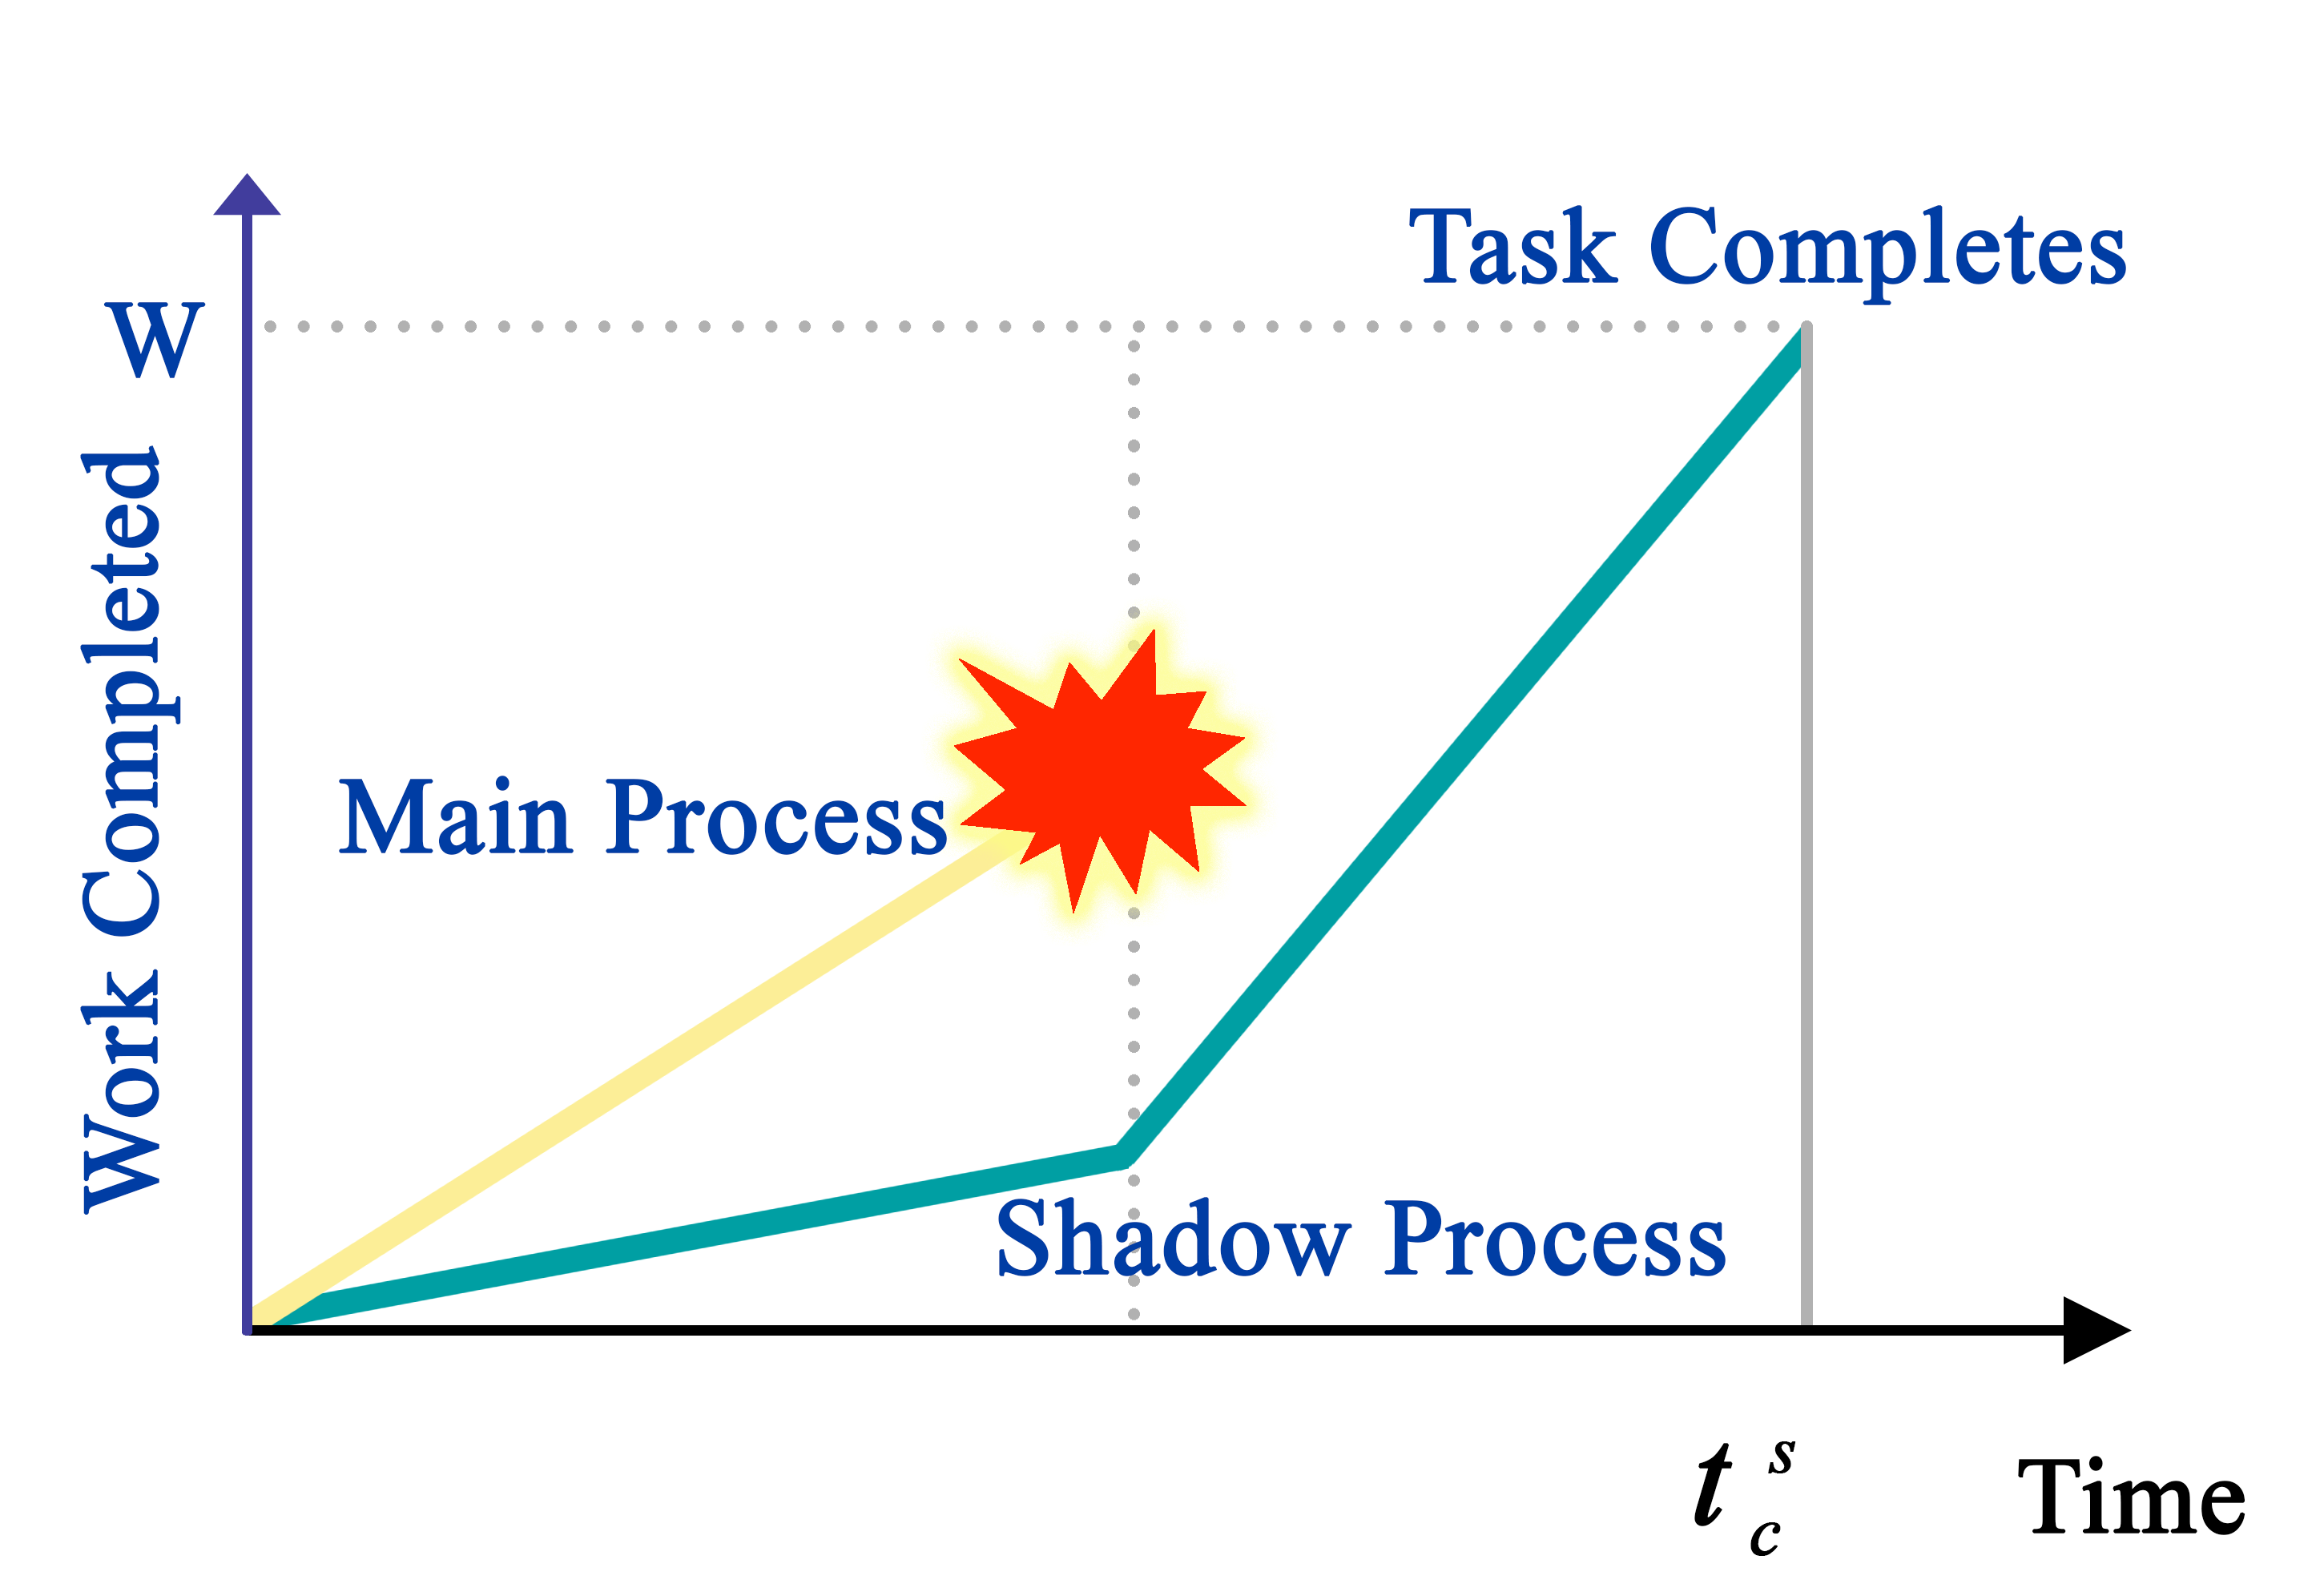
\includegraphics[width=0.33\textwidth]{diagrams/example2.png}
		}
	\end{center}
	\caption{Shadow replication for a single task and single replica}
	\label{fig:sc_overview}
\end{figure*}

\noindent 
The basic tenet of Shadow Replication is to associate with each
main process a suite of ``shadows'' whose size depends on the
``criticality'' of the application and its performance requirements,
as defined by the SLA. 
%To overcome potential failures, the shadows
%execute on separate computing nodes, concurrently with but at slower
%speeds than, the main process.

%The successful completion of the main
%process results in the immediate termination of all shadow
%processes. If the main process fails, the primary shadow process takes
%over the role of the main process and resumes computation, possibly at
%an increased speed, in order to complete the task at a targeted
%response time.


Formally, we define the Shadow Replication fault-tolerance model as follows:
\begin{itemize}
\item A main process, $P_m(W,\text{ }\sigma_m)$, whose responsibility is to executes a task of size $W$ at a speed of $\sigma_m$;
\item A suite of shadow processes, $P_{s}(W,\text{ }\sigma_b^s, \text{ }\sigma_a^s)$ ($1 \le s \le \cal S)$, where $\cal S$ is the size of the suite. 
The shadows execute on separate computing nodes. Each shadow process is associated with two execution speeds. All shadows start execution simultaneously with the main process at speed $\sigma_b^s$ ($1 \le s \le \cal S$). Upon failure of the main process, all shadows switch their executions to $\sigma_a^s$, with one shadow being designated as the new main process. This process continues until completion of the task.
\end{itemize}
%All shadows execute simultaneously with the main process at speed $\sigma_a^s$

To illustrate the behavior of Shadow Replication, we limit the number of shadows to a single process and consider the scenarios depicted in Figure \ref{fig:sc_overview}, assuming a single process failure. Figure \ref{fig:sc_no_fail} represents the case when neither the main nor the shadow fails. The main process, executing
at a higher speed, completes the task at time $t_c^m$. At this time, the shadow process, progressing at a lower speed, stops execution immediately. Figure \ref{fig:sc_shadow_fail} represents the case when the shadow fails. This failure, however, has no impact on the progress of the main process, which still completes the task at $t_c^m$. Figure \ref{fig:sc_main_fail} depicts the case when the main process fails while the shadow is in progress. After detecting the failure of the main process, the shadow begins execution at a higher speed, completing the task at time $t_c^s$. When possible, the shadow execution speed upon failure must be set so that $t_c^s$ does not exceed $t_c^m$. Given that the failure rate of an individual node is much lower than
the aggregate system failure, it is very likely that the main process
will always complete its execution successfully, thereby achieving fault tolerance at a significantly reduced cost of energy consumed by the shadow. %saving a lot of energy for its associated shadow processes. 

%In summary, shadow replication has the following characteristics:
%The proposed shadow replication model has several properties:
%\begin{itemize}
%\item The main process is associated with only one execution speed, $\sigma_m$, %which depends on the size of the task and the SLA requirement.
%\item The shadow processes execute with two different speeds, which are failure %dependent and when possible should be computed to meet the SLA requirement as %closely as possible. 
%\item The completion of the main process results in the immediate termination of %all shadow processes. Given that the failure rate of an individual node is much %lower than the aggregate system failure, it is very likely that the main process %completes successfully, saving a significant amount of energy, while achieving %high level of fault tolerance.
%\end{itemize}



A closer look at the model reveals that shadow
replication is a generalization of traditional fault tolerance
techniques, namely re-execution and traditional replication. If the
SLA specification allows for flexible completion time, shadow
replication would take advantage of the delay laxity to trade time
redundancy for energy savings. It is clear, therefore, that for a
large response time, Shadow Replication converges to re-execution, as
the shadow remains idle during the execution of the main process and
only starts execution upon failure. If the target response time is
stringent, however, Shadow Replication converges to pure replication,
as the shadow must execute simultaneously with the main at the same
speed. The flexibility of the Shadow Replication model provides the
basis for the design of a fault tolerance strategy that strikes a
balance between task completion time and energy saving, thereby
maximizing profit.

Given that the probability of two individual nodes executing the same
instances of a task fail at the same time is low, we will focus on the study of Shadow Replication model with a single shadow. It is clear, however, that the model can
be extended to support multiple processes, as required by the
application's fault-tolerance requirement. Furthermore, we adopt the
fail-stop~ fault model, where a processor stops execution once a fault
occurs and failure can be detected by other
processes\cite{gartner_faults_1999,cristian_comm_1991}.

%While all
%shadow processes are exact replicas of the main process, one among
%these processes, referred to as primary shadow process, is special in
%that it would become new main process if current one fails.

% stated in paragraph one now.
%In order to mask failure during a task,
%the shadow processes are scheduled to execute concurrently with the
%main process, but on different computing nodes. Furthermore, in order
%to reduce energy, shadow processes initially execute at decreasingly
%lower processor speeds.


%Moreover, one among the remaining shadow processes is promoted
%to primary shadow process. By allowing instantaneous fail-over with
%shadow processes in the event of failure, shadow replication eliminates
%even the smallest chance of data loss or disruption.


%Without loss of generality, from this point on we
%assume at most one failure would occur to a task and consider a dual
%level of redundancy, whereby only one shadow process is executed
%concurrently with each main process. The completion of the main or its
%shadow results in the successful execution of the task. If the main
%process fails, it is implied that shadow process would complete the
%task.



% needless words
%Figure \ref{fig:sc_overview} depicts how shadow replication works to
%complete a single task using a single replica. While the main process
%would execute at a certain fixed speed until task completion or
%failure, the shadow process may change its speed if it needs to take
%over the role of main process, in order to finish task in
%time. According to if and when failure occurs, there are three cases
%that may happen during the execution of the task.


%In this section we have defined shadow replication and described its
%potential in energy saving and profit gain in cloud computing
%environment. Three questions, however, remain to be answered before we
%expect shadow replication to be accepted as a novel fault tolerance
%technique for cloud computing: 1) is it truly possible for shadow
%computing to save energy and bring more profit over state-of-the-art
%fault tolerance approaches while meeting SLA requirements; 2) if so,
%how much benefit can it bring; 3) how to determine the optimal
%execution speeds for main process and shadow processes.
%
%To answer the above questions, in the following section we will
%introduce a reward-based analytical model for fault tolerance
%mechanisms with a dual-level redundancy under the assumption that at
%most one process may fail.
